\documentclass{standalone}
\usepackage{tikz,ctex}
\usepackage{tikz-3dplot} % 2-1
\usepackage{unicode-math} % 2-5,4-1,4-2
\setmathfont{Fira Math Regular}
\setmainfont{Fira Sans}
\definecolor{background}{RGB}{239, 239, 239} % 4-5,6-2,6-5
\begin{document}
\usetikzlibrary{calc}
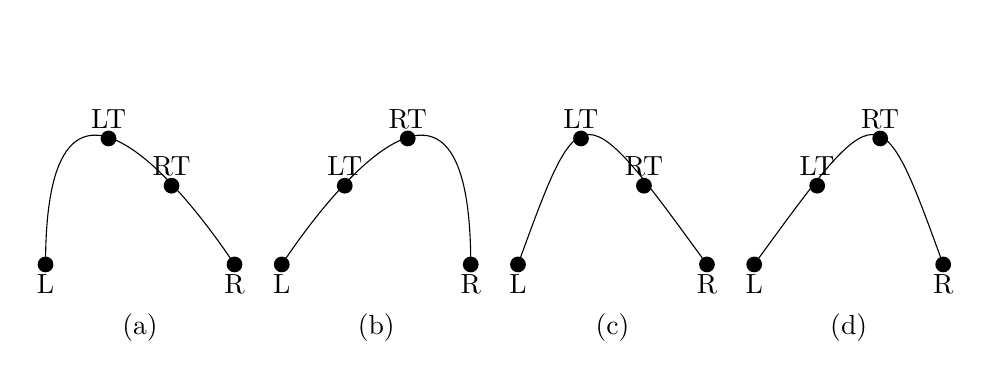
\begin{tikzpicture}
\foreach \x in {0,1,2,3}{  
    \fill   ($(0,0)!\x*.25!(12,0)$) circle (.1) node[below]{L}
            ($(2.4,0)!\x*.25!(14.4,0)$) circle (.1) node[below]{R}
            ($(0.8,0)!\x*.25!(12.8,0)!abs(cos(\x*90))*.3+.5!(0.8+3*\x,2)$) circle (.1) node[above]{LT}
            ($(1.6,0)!\x*.25!(13.6,0)!abs(sin(\x*90))*.3+.5!(1.6+3*\x,2)$) circle (.1) node[above]{RT};}
\draw (0,0) ..controls (0,3) and (1.6,1.2)..(2.4,0);
\draw (5.4,0) ..controls (5.4,3) and (3.8,1.2)..(3,0);
\draw (6,0) ..controls (6.8,2.2)..(8.4,0);
\draw (11.4,0) ..controls (10.6,2.2)..(9,0);
\foreach \i[count=\x] in {a,...,d}{
    \node at(3*\x-1.8,-.8){(\i)};}
\end{tikzpicture}
\end{document}